\documentclass[
  shortnames]{jss}

\usepackage[utf8]{inputenc}

\providecommand{\tightlist}{%
  \setlength{\itemsep}{0pt}\setlength{\parskip}{0pt}}

\author{
Shannon K. Gallagher\\Biostatistics Research Branch\\
National Institute of Allergy\\
and Infectious Diseases \And Benjamin LeRoy\\Dept. of Statistics \& Data Science\\
Carnegie Mellon University
}
\title{Time invariant analysis of epidemics with \pkg{EpiCompare}}

\Plainauthor{Shannon K. Gallagher, Benjamin LeRoy}
\Plaintitle{Time invariant analysis of epidemics with EpiCompare}
\Shorttitle{\pkg{EpiCompare}}

\Abstract{
We present \pkg{EpiCompare}, an \proglang{R} package that suppliments
and enhances current infectious disease analysis pipelines and
encourages comparisons across models and epidemics. A major contribution
of this work is the set of novel \textit{time-invariate} tools for model
and epidemic comparisons - including time-invariate prediction bands.
\pkg{EpiCompare} embraces \proglang{R}'s \textit{tidy} coding style to
make adoption of the package easier and analysis faster. This paper
provides an overview of both the tools in and intuition behind
\pkg{EpiCompare} and a thorough demonstrating of the tools through a
detailed example of a full data analysis pipeline.
}

\Keywords{keywords, not capitalized, \proglang{Java}}
\Plainkeywords{keywords, not capitalized, Java}

%% publication information
%% \Volume{50}
%% \Issue{9}
%% \Month{June}
%% \Year{2012}
%% \Submitdate{}
%% \Acceptdate{2012-06-04}

\Address{
    Shannon K. Gallagher\\
    Biostatistics Research Branch\\
  National Institute of Allergy\\
  and Infectious Diseases\\
    5603 Fishers Lane\\
Rockville, MD 20852\\
  E-mail: \email{shannon.gallagher@nih.gov}\\
  URL: \url{http://skgallagher.github.io}\\~\\
      Benjamin LeRoy\\
    Dept. of Statistics \& Data Science\\
  Carnegie Mellon University\\
    5000 Forbes Ave.\\
Pittsburgh, PA 15213\\
  E-mail: \email{bpleroy@andrew.cmu.edu}\\
  URL: \url{https://benjaminleroy.github.io/}\\~\\
  }


% Pandoc header
\usepackage{booktabs}
\usepackage{longtable}
\usepackage{array}
\usepackage{multirow}
\usepackage{wrapfig}
\usepackage{float}
\usepackage{xcolor}
\usepackage{rotating}

\usepackage{amsmath} \usepackage{amssymb} \usepackage{amsthm} \usepackage{afterpage} \usepackage[normalem]{ulem}

\begin{document}

\newcommand{\shannon}[1]{\textcolor{orange}{#1}}
\newcommand{\shan}[1]{\textcolor{brown}{#1}}
\newcommand{\ben}[1]{\textcolor{violet}{#1}}

\newtheorem{theorem}{Theorem}

\section[Intro]{Introduction}\label{sec:intro}

The recent (and on-going) COVID-19 global pandemic has galvanized public
interest in understanding more about infectious disease modeling and has
highlighted the usefulness of research in the area of infectious disease
epidemiology. Infectious diseases inflict enormous burdens on the world:
millions of lives lost and trillions of dollars spent yearly. Infectious
disease models typically attempt to do one or more of the following: 1)
predict the spread of current and future epidemics
\citep[e.g. flu prediction][]{Biggerstaff2016}, 2) analyze past and
current epidemics to increase scientific knowledge
\citep[e.g. historical measle outbreaks][]{Neal2004}, and 3) forecast or
project epidemic scenarios under pre-specified parameters
\citep[e.g.][]{ferguson2020}. At the same time, descriptive statistics
and visualizations from universities, many branches and levels of
government, and news organizations are an important first step of the
process, as has been seen in the current COVID-19 pandemic
\citep{dong2020,cdc-covid-tracker2021,wp-covid-tracker2021}.

With many visualization and exploratory tools, models and modeling
paradigms, and reviews and comparisons in the literature and through the
MIDAS (Models of Infectious Disease Agent Study) network
\citep{midasnetwork2021} available, this field has a number of devices
to \textcolor{orange}{\sout{aid}}
\textcolor{orange}{help}\footnote{\textcolor{violet}{[Ben says: I'm not sure this an improvement]}}
an individual practitioner decide the correct approach. For example,
\proglang{R} packages such as \pkg{surveillance}, \pkg{EpiModel}, and
\pkg{pomp} have all made significant steps in standardizing the flow of
the data analysis pipeline for epidemic modeling through digitizing data
sets, making accessible statistical models, and providing a plethora of
educational material for both coding novices and experts alike
\citep{surveillance2017,Jenness2018,King2016}.

At the same time, analysis packages often only address a specific
portion of the analysis pipeline. These modeling tools usually require
learning package-specific syntax and often don't provide easy ways to
compare and assess their models on new data. Moreover, exploring
modeling and comparing epidemics require transforming and
\textit{tidying} data in different ways. To fill these gaps, we present
our \proglang{R} package \pkg{EpiCompare}. Our package's primary focus
is to aid and advance research in the area of comparison and assessment
of epidemic and epidemiological models. In Figure \ref{fig:pipeline}, we
illustrate the data analysis pipeline of infectious diseases as 1) data
pre-processing, 2) exploratory data analysis (EDA), 3) modeling and
simulating, 4) post-processing, and 5) comparison and assessment; where
each previous part of the pipeline influences the next. \pkg{EpiCompare}
provides tools to aids practitioners in all areas of this pipeline.

\begin{figure}[!ht]
    \centering
    \includegraphics[width = 1\textwidth]{images/pipeline1.png}
    \caption{An idealized epidemiological data analysis pipeline.}
    \label{fig:pipeline}
\end{figure}

One of \pkg{EpiCompare}'s main contribution to comparison and assessment
of epidemics is through tools that provide \textit{time-invariant}
assessments. Epidemics, despite being defined as a process that evolves
over time, often need to be compared in a way not constrained to initial
times or time scales in order to understand the processes at play. With
time-invariant analysis, comparing decades-long outbreaks of HIV in the
US to a 10 day outbreak of norovirus on a cruise ship is possible.
Compared to time-dependent comparison tools for state-space modeling,
time-invariant analysis can make it easier to compare state-space
epidemic representations in a more global, holistic fashion. Many
time-dependent comparison tools only examine the proportion of
individuals in each state (at a given time) in a piece-wise / marginal
fashion. These time-dependent approaches can reduce the amount of
connections that can be seen and insights that can be drawn\}, similar
to examining projections of a multidimensional distribution onto a
single axis, one at a time. Tools in \pkg{EpiCompare} extend the user
toolkit to evaluate epidemics within a time-invariant lens. At the same
time, the goal of \pkg{EpiCompare} is not to supplant existing
infectious disease modeling tools and software but, rather, is a
concerted effort to create standard and fair comparisons among models
developed for disease outbreaks and outbreak data.

This paper is broken up into the following sections; section
\ref{sec:time-invariant} motivates and showcases tools of time-invariant
analysis, section \ref{sec:overview} presents an outline of how
\pkg{EpiCompare} aids a practitioner in every step of the pipeline and
section \ref{sec:tour} provides a demonstration of the tools through a
detailed
example\textcolor{orange}{\sout{ of a full data analysis pipeline.}}
\textcolor{orange}{from start to finish of the data analysis pipeline}\footnote{\textcolor{orange}{maybe clearer? up to you} \textcolor{violet}{The current suggestion isn't clearer - feel free to try again.}}

\hypertarget{sec:time-invariant}{%
\section{Time-invariant analysis}\label{sec:time-invariant}}

\pkg{EpiCompare} emphasizes the value of analyzing epidemics in a
\textit{time-invariant} way - approaches that remove some or all of the
impact of start/end times and recording time scales when preforming the
analysis. In this section we highlight some weaknesses of
time-\textit{de}pendent analysis and define the mathematical
underpinning of the time-invariant approach we take. To accomplish this
goal we first demonstrate the inability of time-dependent tools to
adequately quantify a classic epidemic parameter, the reproduction
number \(R_0\). Then we motivate new time-invariant approaches for more
complex situations where \(R_0\) does not capture the complexities of
outbreaks. This leads to the final subsection that defines ways to view
epidemics in a time-invariant lens and discusses natural properties of
these representations that allow for clearer ways to compare models and
epidemics.

\subsection[Motivation through the reproduction number $R_0$]{Motivation
of time-invariant analysis through the reproduction number
\(R_0\)}\label{sec:r0_subsection}

Epidemiological research is often interested in understanding intrinsic
properties of the epidemic, independent from when the epidemic occurred
or how frequently data was collected. One of the most famous numerical
summaries of an epidemic is the reproduction number - \(R_0\). This
numerical summary is a time-invariant value that is defined as the
expected number of infections caused by a single infect or who is added
to a completely susceptible population \citep{anderson1992}.
\citet{Gallagher2020} showed that the estimation of \(R_0\) can be
sensitive to time-dependent parameters like estimation of the beginning
and end of an epidemic. This time-dependent sensitivity in estimating
\(R_0\) reflects a general problem in epidemiology surrounding how to
transform time-dependent information into insights into desirable,
intrinsic properties of an epidemic.

In many situations, epidemiologists want a much deeper understand of an
epidemic than just the reproduction number. One common time-dependent
tool used to better understand epidemics is a series of time series line
plots that track the proportion of the population in a given state
(e.g.~infected) at a given time. Figure
\ref{fig:different-scales-standard} visualizes two different simulated
epidemics with population states (S)usceptible, (I)nfectious and
(R)ecovered. These simulations have been generated under a discrete
approximation of \citet{Kermack1927}'s SIR model. The Kermack and
McKendrick model captures the transitions from one state to the next as
a system of ordinary differential equations

\begin{align}\label{eq:sir-ode}
    S^\prime(t) &= -\frac{\beta S(t)I(t)}{N} \\
    I^\prime(t) &= \frac{\beta S(t)I(t)}{N} - \gamma I(t) \nonumber\\
    R^\prime(t) &= \gamma I(t) \nonumber,
\end{align}

where \(N\) is the total number of individuals, \(\beta\) is the rate of
infection, and \(\gamma\) is the rate of recovery.

From this model, the reproduction number is the ratio of the infection
rate to the recovery rate, \(R_0 = \beta/\gamma\).

\begin{CodeChunk}
\begin{figure}[H]

{\centering 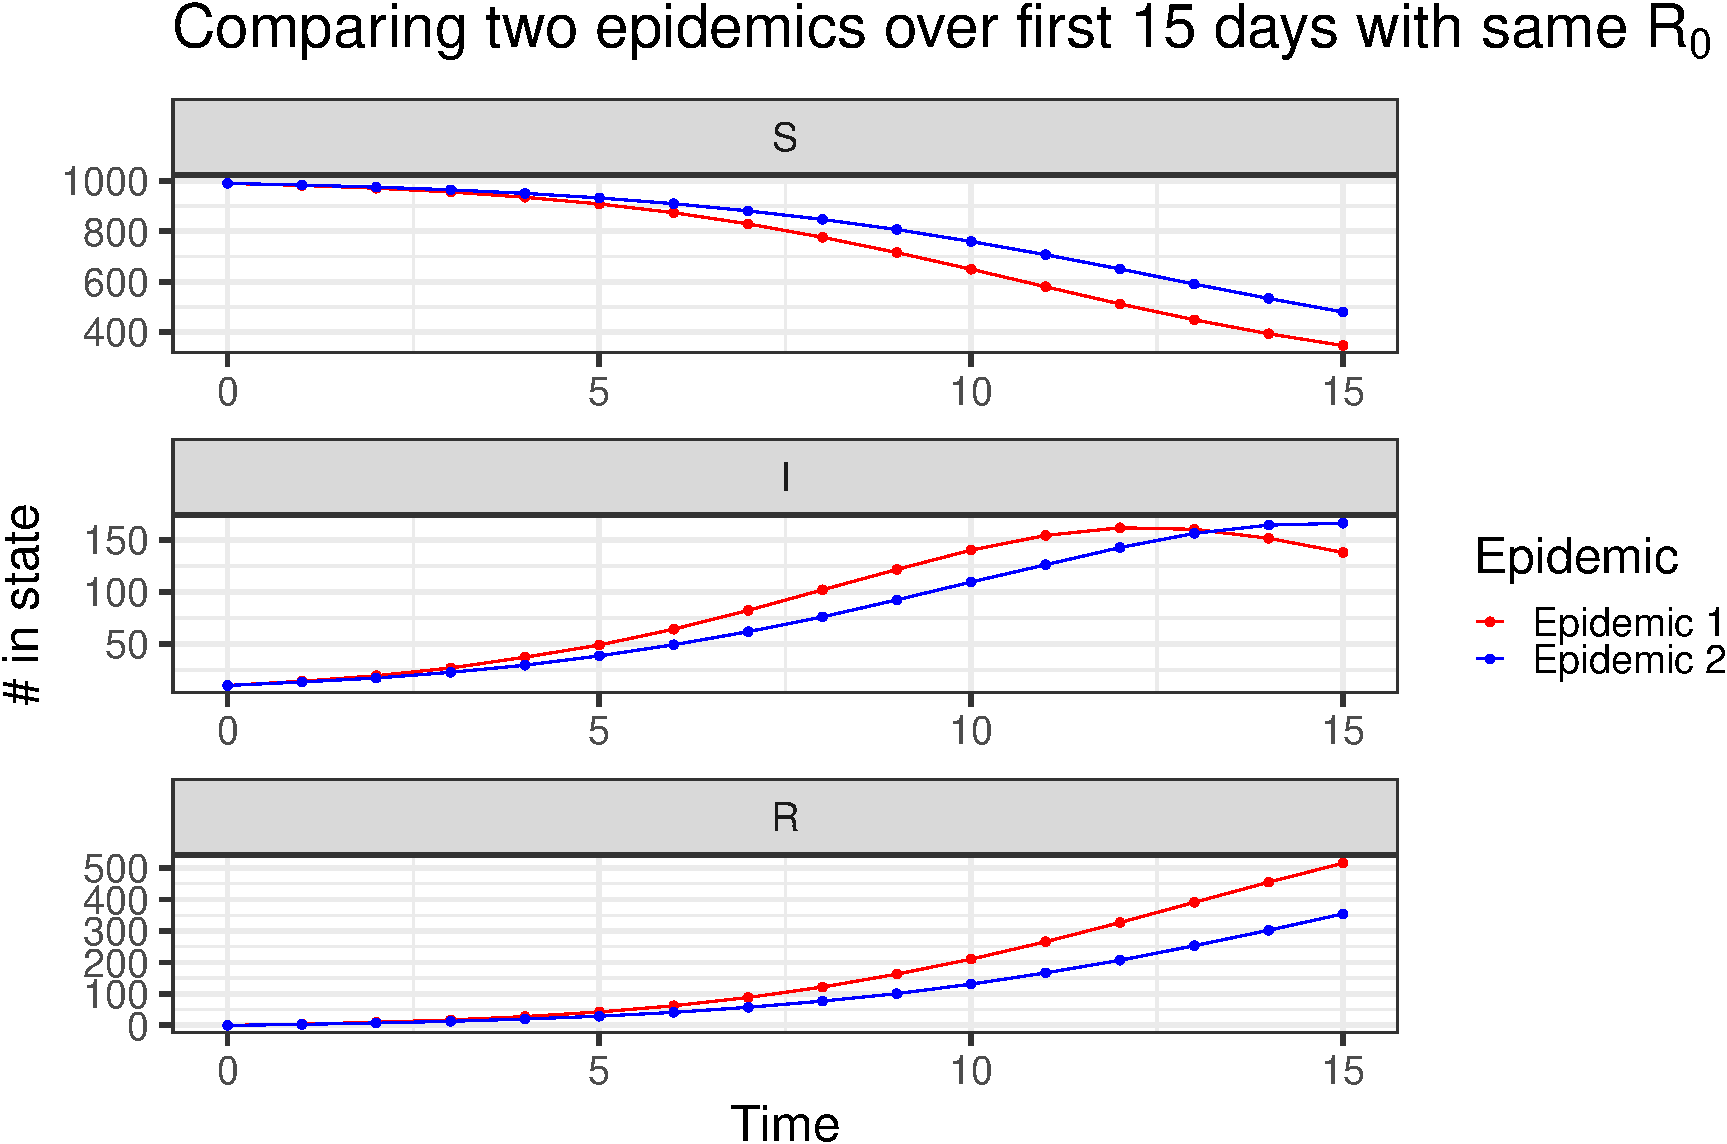
\includegraphics{Figs/unnamed-chunk-2-1} 

}

\caption{\label{fig:different-scales-standard}Example of two epidemics with different $\beta$ and $\gamma$ parameters but the same initial reproduction number $R_0$ = 2.  Both epidemics are generated from models with $N= 1000$ individuals with $S(0) = 990$ and $I(0) = 10$.}\label{fig:unnamed-chunk-2}
\end{figure}
\end{CodeChunk}

Even though Figure \ref{fig:different-scales-standard}'s visual analysis
might be able to present more complex properties of the epidemic, one
might wish to understand how these two simulated epidemics' \(R_0\)
values compare. Even though these two simulated epidemics appear
different in these figures (including having different infection peaks),
there is no real intuitive way to compare the epidemics' \(R_0\) values.
In fact, both of these simulated epidemics started with the same
population (1000 total people with 10 infected) and have the same
\(R_0\) value, just with slightly different infection and recovery rates
(\(\beta_1, \gamma_1 = 0.8, 0.4\), and
\(\beta_2, \gamma_2 = .64, .32\)). Even for simple generative models,
this time-dependent visualization cannot be used to compare a very
simple but powerful numerical summary, \(R_0\).

\hypertarget{ternary-plots-a-time-invariant-visualization-tool}{%
\subsection{Ternary plots: a time-invariant visualization
tool}\label{ternary-plots-a-time-invariant-visualization-tool}}

The faceted time series plot, like that seen in Figure
\ref{fig:different-scales-standard}, not only fails to allow the
practitioner to compare simulated epidemics' \(R_0\) values but also
presented epidemics' trajectory data so that only the marginal
information for each state can be examined at a given time. A more
holistic approach to visualizing the overall path of our simulated
epidemics is to examine how each epidemic traverses the
three-dimensional \((S(t),I(t),R(t))\) space. Figure 3's left plot does
just that, presenting the trajectories of the simulated epidemics in
this three-dimensional space. For state space models like in our
example, given the constraint that \(S(t) + I(t)+R(t)\) is always equal
to \(N\) (the total population size) we can visual these point in a a
two-dimensional \textit{ternary} plot, as seen in Figure
\ref{fig:different-scales-tern}'s right plot. In both of Figure
\ref{fig:different-scales-tern}'s plots we observe that the two
epidemics are on the same trajectory. In this simple generative example
setting, being on the same trajectory indicates that the two epidemics
have the same \(R_0\) value. This can be proven mathematically.

\begin{CodeChunk}
\begin{figure}[H]

{\centering 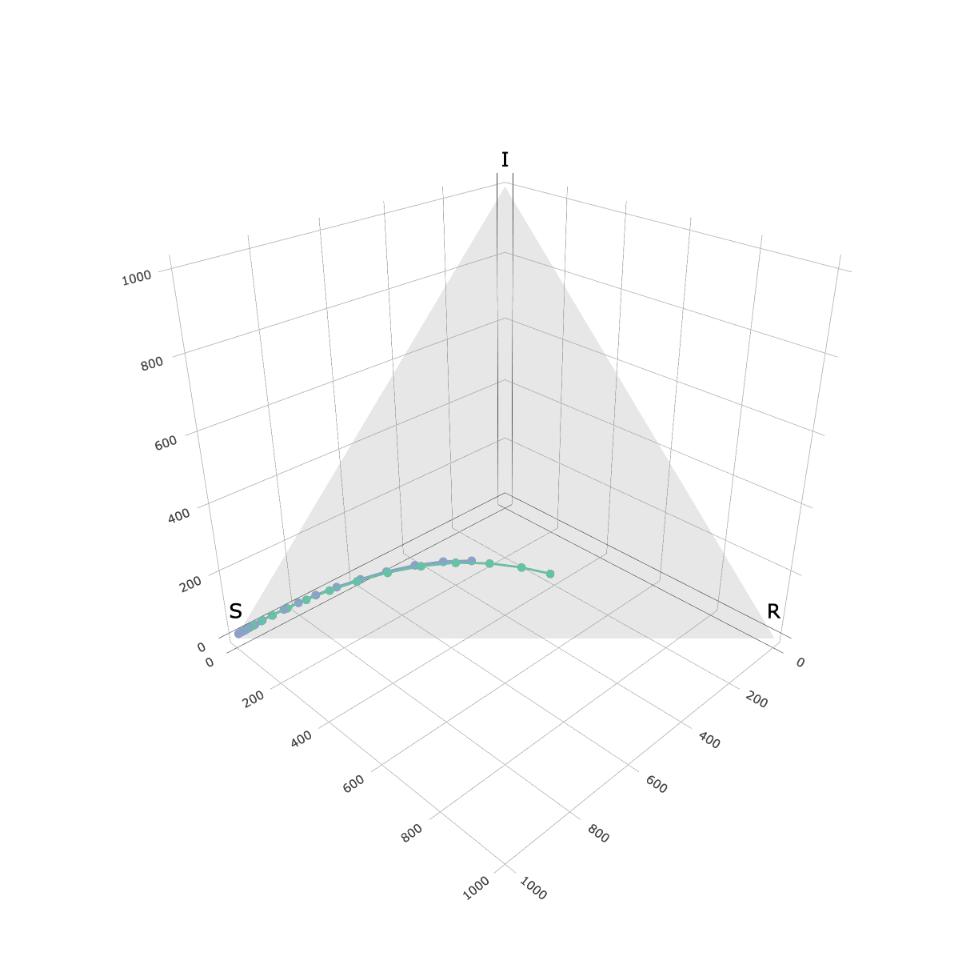
\includegraphics[width=0.49\linewidth]{images/vis3d} 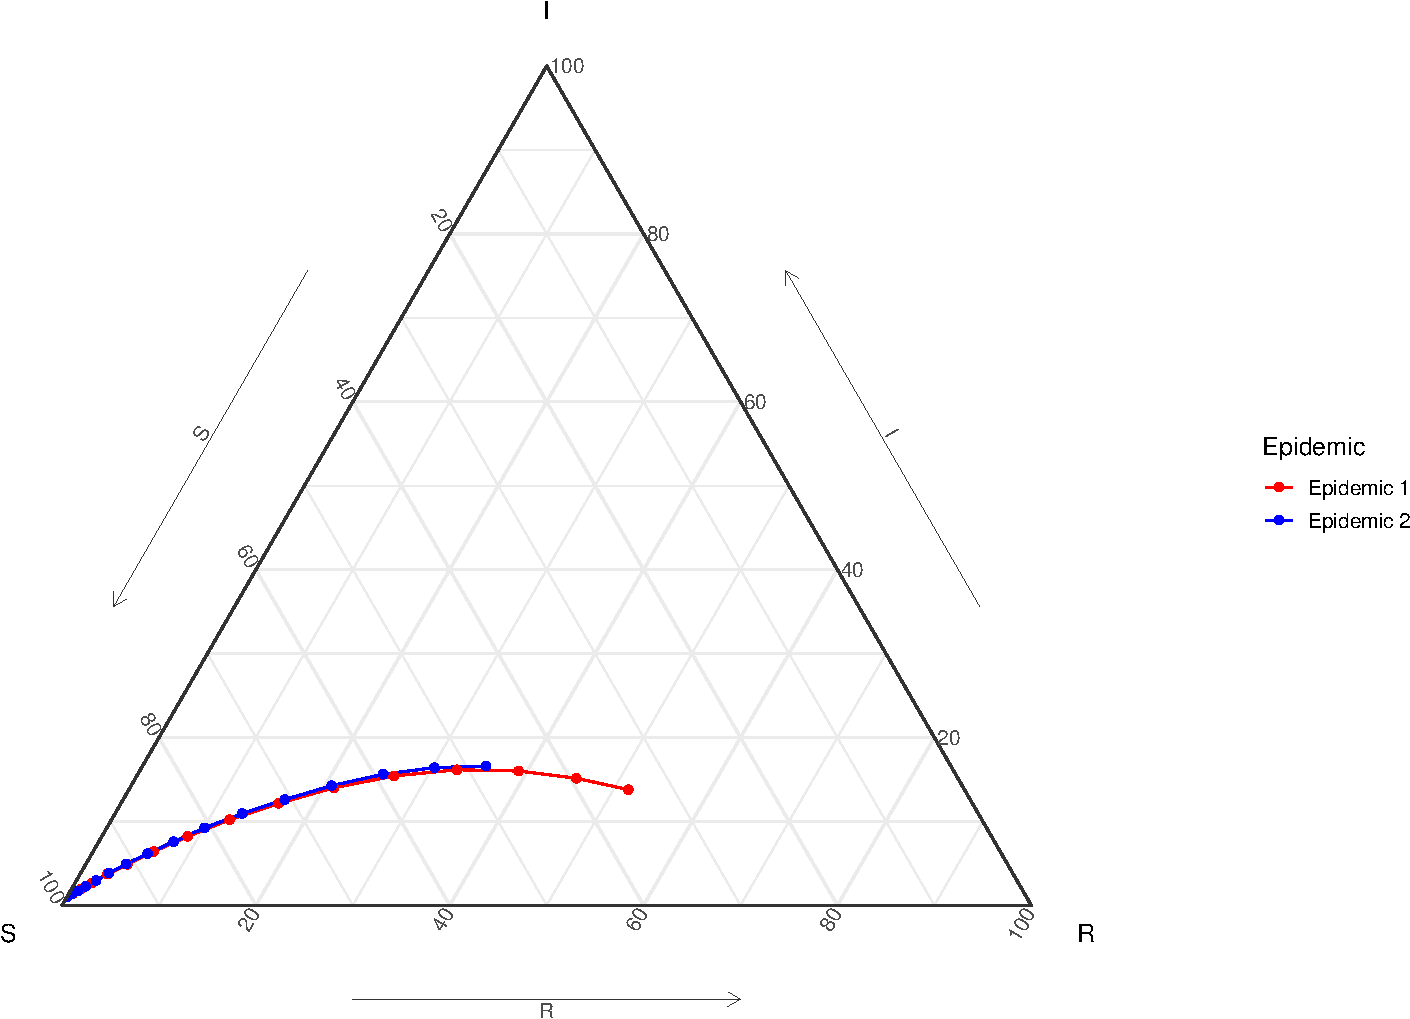
\includegraphics[width=0.49\linewidth]{Figs/unnamed-chunk-3-2} 

}

\caption{\label{fig:different-scales-tern}Left: trajectory of epidemic in three-dimensional space, plotting $(S(t), I(t), R(t))$.  Right: the gray-shaded region and epidemic trajectories shown from (left) now shown in two-dimensional space.  This is more commonly known as a ternary plot.}\label{fig:unnamed-chunk-3}
\end{figure}
\end{CodeChunk}

\begin{theorem}\label{thm:sir-scale}
 Let there be two \citet{Kermack1927}'s SIR models ($(S_1(t),I_1(t),R_1(t))_{t\geq 0}$ and $(S_1(s),I_1(s),R_1(s))_{s\geq 0}$), with $(S_1(0),I_1(0),R_1(0))=S_2(0),I_2(0),R_2(0))$  Let both models have the same $R_0$ (i.e. $R_0 = \frac{\beta_1}{\gamma_1} = \frac{\beta_2}{\gamma_2}$) and define $a > 0$ such that $\beta_2 = a\beta_1$. Then for all $t > 0$ there exists $s>0$ such that $(S_1(t), I_1(t), R_1(t)) = (S_2(s), I_2(s), R_2(s))$.  Moreover, $s = \frac{1}{a}t$.
\end{theorem}

The proof of Theorem \ref{thm:sir-scale} relies on a fairly recent
result from \cite{Harko2014} and is shown in detail in Proof
\ref{proof:thm}. The consequence of Theorem \ref{thm:sir-scale} is that
for two SIR models that have the same initial percent of individuals in
each state and \(R_0\), then every point on the epidemic path of the
first SIR model can be mapped to a point on the epidemic path of the
second SIR model. In other words, the two epidemics form the same
filamental trajectory.

\hypertarget{time-invariance-beyond-sir-models-trajectories-and-filaments}{%
\subsection{Time-invariance beyond SIR models: Trajectories and
Filaments}\label{time-invariance-beyond-sir-models-trajectories-and-filaments}}

Through the \(R_0\) example, we see that treating epidemics like
filamental trajectories embedded in a lower dimensional space allows us
to better compare the overall structure of the epidemic and see how the
population is directly impacted. In this section we present
time-invariant tools that can be applied to complex epidemics where the
epidemic's generative process is unknown and can have more than three
states. These tools leverage the idea that an epidemic can be viewed as
a trajectory and that many properties of the epidemic are well captured
when we do so. This approach is useful when the epidemic of interest has
only gone through a single realization of its outbreak (before the
population of individuals become susceptible again).

The first set of tools allows a practitioner to define distances between
epidemics whose time features do not align. For completed epidemics, one
way to better examine their properties is to represent their filamental
trajectories as a finite sequence of equally spaced points. This
representation induces a natural distance between epidemics,
specifically:

\[
d_\text{equi-distance}(\psi_1, \psi_2)  = \int_{s \in [0,1]} (\tilde{\psi}_1(s) - \tilde{\psi}_2(s))^2 ds \nonumber,
\] where \(\tilde{\psi}_i(s)\) is the point along \(\psi_i\) that is
\(s\cdot|\psi_i|\) distance away from the start of \(\psi_i\) (with
\(|\psi_i|\) is the length of \(\psi_i\)). This distance is naturally
time-invariant, and can be plugged into multiple distance-based
assessment tools to examine the overall ``extremeness'' of points,
including pseudo-density estimators and depth/local depth functions
\citep[for examples see][]{Ciollaro2016, Geenens2017}. These extremeness
estimators can be useful when comparing the true epidemic to a set of
simulated epidemics, and practitioners can interpret the epidemic's
extremeness score relative to the extremeness scores of the simulations
very easily.

In addition to being used to better understand completed epidemics,
time-invariant tools can be used to aid prediction of future epidemics
by providing a state-space regions in which we expect the true epidemic
to traverse. In settings where the epidemic only generates a single
outbreak, these regions can be very telling if simulation models capture
the epidemic's structure. In \pkg{EpiCompare} we create geometric
prediction regions around all but the \(\alpha\) proportion of most
extreme simulated trajectories. These geometric regions can also be used
to compared simulation models that have different time scales,
parameters and even different statistical philosophies, through set
different distances. Although visualization is the easiest when the
epidemic has three states, prediction regions can be useful to assess
and compare simulation models where the epidemics have multiple states.

Overall, there are many tools to aid in the assessment and comparison of
epidemics and models that avoid being affected by time-based parameters.
We believe the time-invariant analysis provides many insights and should
be in the toolkit of many epidemiologists. \pkg{EpiCompare} provides a
strong starting point to do just that.

\section[Package overview]{Overview of
\pkg{EpiCompare}}\label{sec:overview}

\afterpage{\clearpage}
\begin{sidewaysfigure}[!ht]
    \centering
    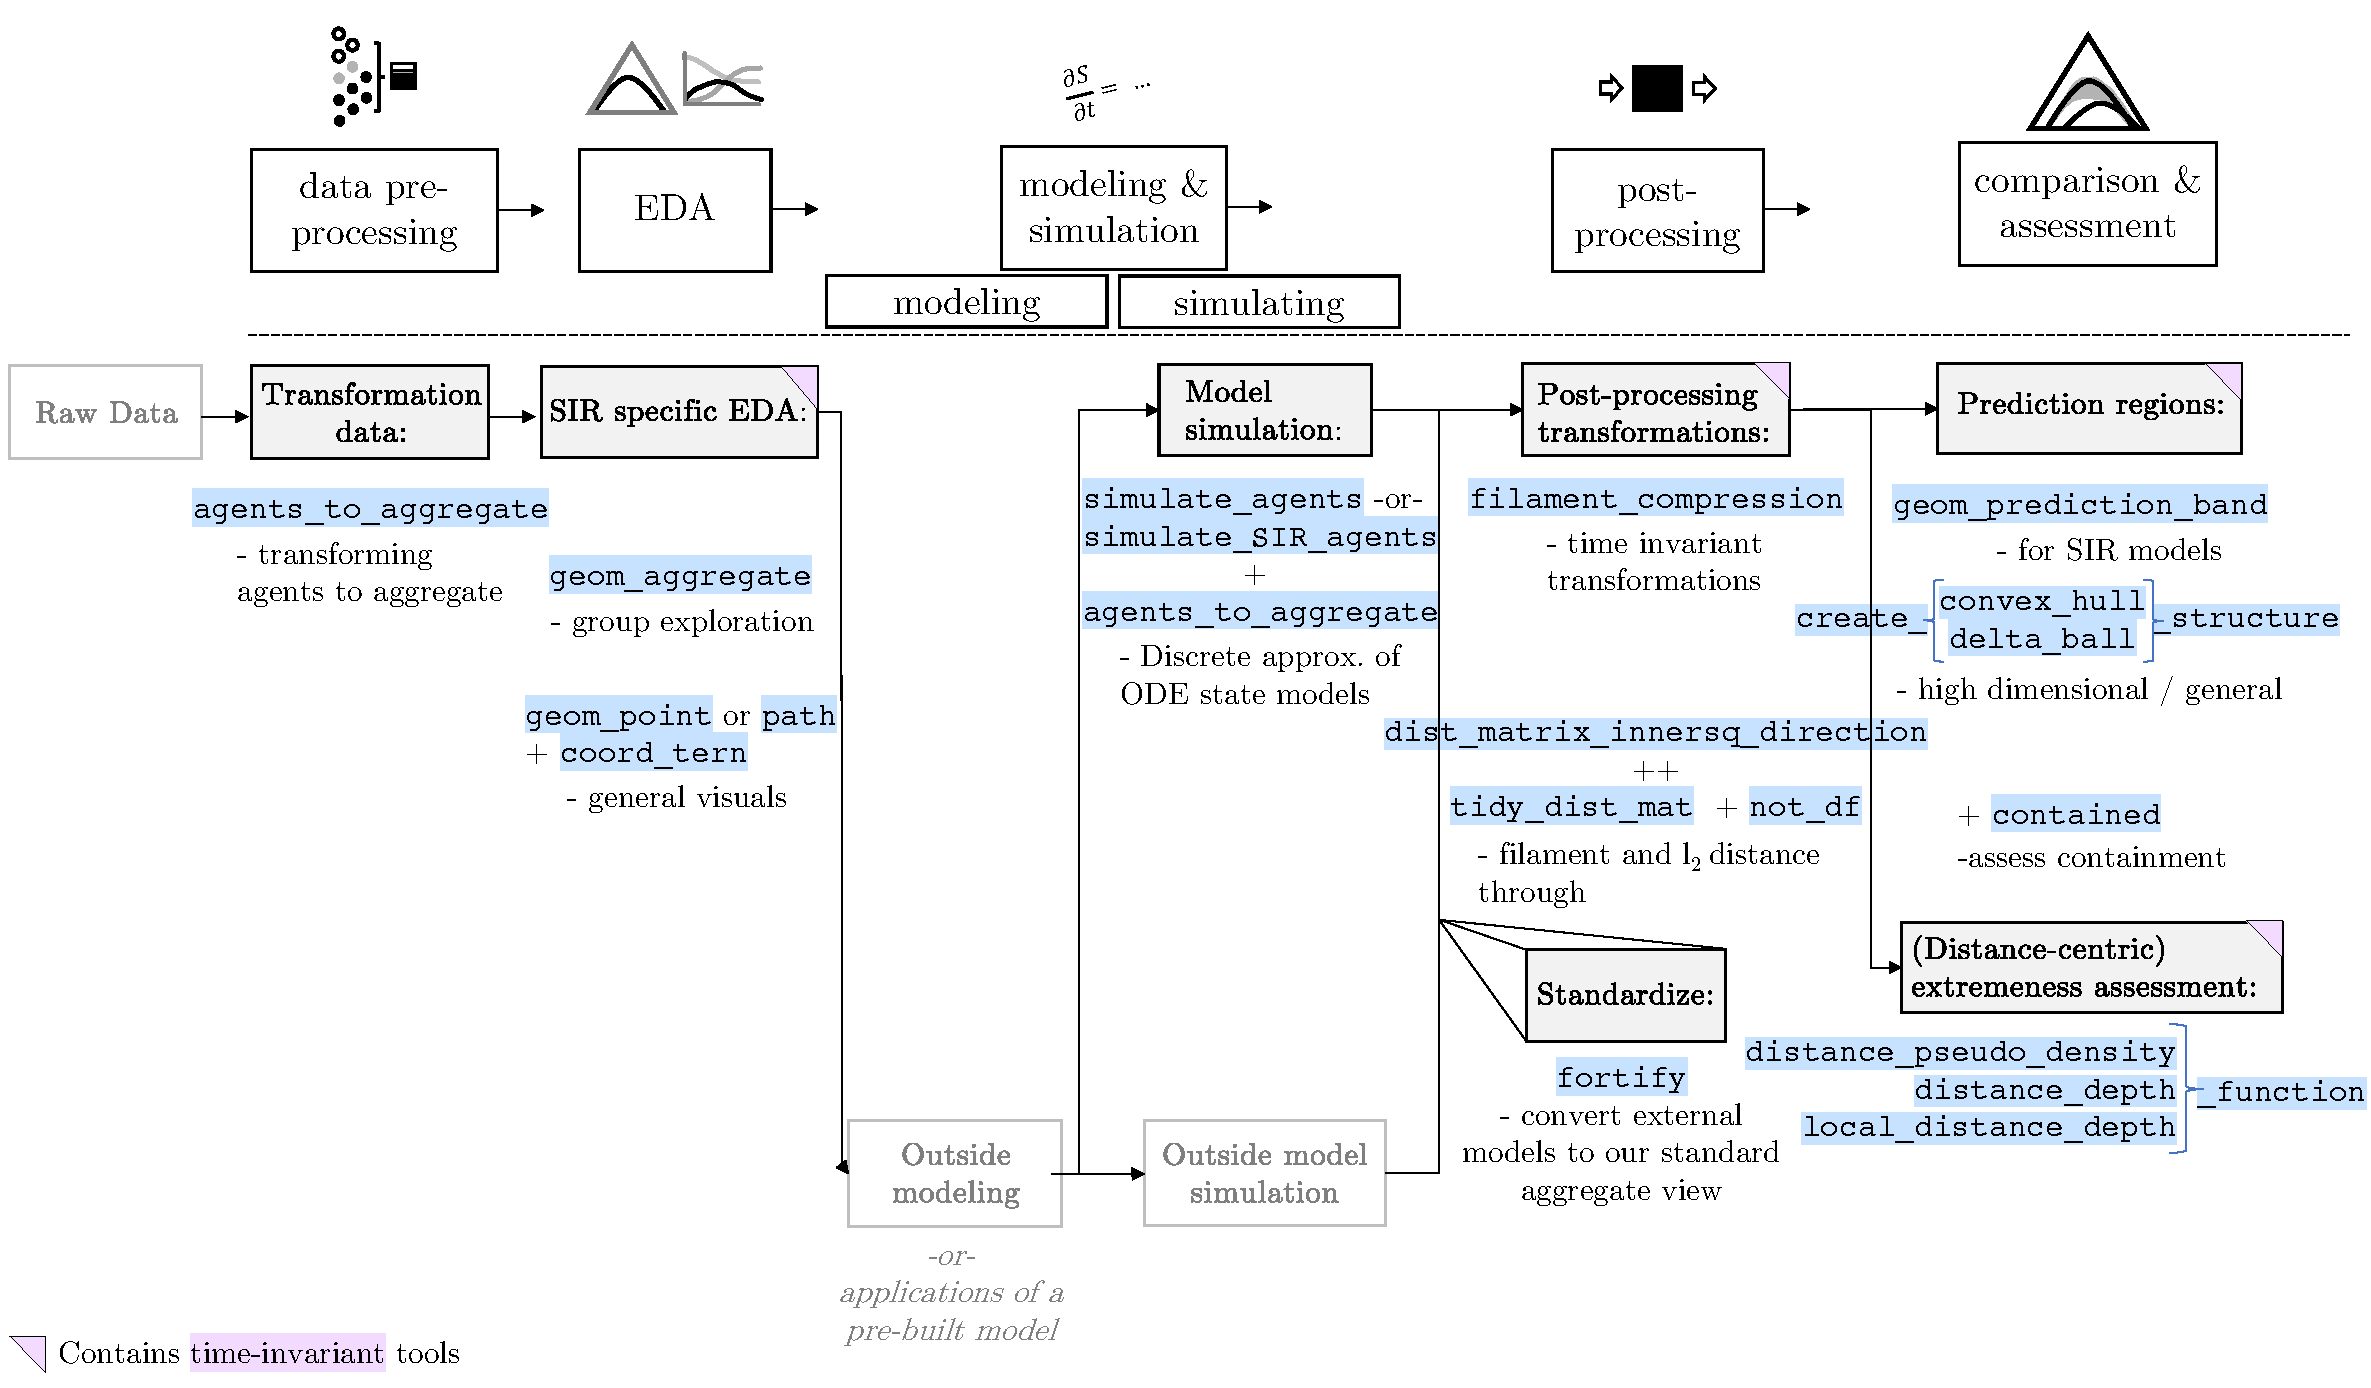
\includegraphics[width = 1\textwidth]{images/pipeline2_2.pdf}
    \caption{How \pkg{EpiCompare} supplements and aids in the epidemiological data analysis pipeline.}
    \label{fig:pipeline2}
\end{sidewaysfigure}

In this section, we present the tools implemented in \pkg{EpiCompare}
and explain how they aid in the data analysis pipeline. In Fig.
\ref{fig:pipeline2}, we illustrate how our package's functions fit into
the data analysis pipeline introduced in Fig. \ref{fig:pipeline}. All
front-facing functions are aimed to be as user-friendly as possible. We
also focus on providing the user ``tidyverse'' style functions, that
encourage piping objects from one function to the next and follow clear
``verb'' naming schemes \citep{Wickham2019}. Although users can
incorporate \pkg{EpiCompare} into any step in the data analysis
pipeline, there are two primary points of entry. The first point of
entry is the very beginning with pre-processing and visualizing raw
data, and the second point of entry is after modeling and simulation.
Figure \ref{fig:pipeline2} captures these different paths, and we
highlight\footnote{\textcolor{violet}{[Ben says: we need to make sure we actually do highlight ]}}
both approaches and how to leverage \pkg{EpiCompare} in the subsections
below.

\textbf{Data Pre-processing}

The first step of most data analysis is ``cleaning'' the data
\textcolor{orange}{to a format that is friendly for both computers and programmers}\footnote{\textcolor{violet}{[Ben says: I'm unsure this is needed and naturally adds more text. Willing to accept...]}\textcolor{brown}{When in doubt, remove.}}
so it can be explored.
\sout{There are multiple ways to collect epidemiological data.}
\textcolor{violet}{In epidemology, there are multiple different formats the data can arrive in.}
\footnote{\textcolor{orange}{[Shannon suggests: "Epidemiological data are collected in many different formats."]} \textcolor{violet}{[Ben says: I see the point you're trying to make and made a new edit - but it's less connected to the previous sentence since "format" is the end.]}\textcolor{brown}{What about adding a linking sentence "Before data can be explored, it must be colleected.  Epidemiological data are collected in many different formats."}}
Sometimes individual records are collected, with times of different
states of the epidemic (infection, recovery, etc.) as well as individual
information like network structure, location, and sub-population
information. Other data collections focus on aggregate counts of
individuals in each epidemic state. In fact, many times only the number
of new infections at each time step (e.g.~weekly case counts) is
observed. Compartment totals (amounts of individuals in each state) are
then imputed from those case
counts\sout{ along with}\textcolor{orange}{and}\footnote{\textcolor{violet}{[Ben says: Declined. I'm unclear why we should. Is the sentence unclear? Maybe it's the way it's a compound sentence? - If so a rewrite would be better?]}\textcolor{brown}{Upon reflection, I think it's fine.}}
other information about the disease and the population of interest. In
\pkg{EpiCompare}, we focus on understanding the overall impact of an
outbreak at the aggregate/population level, which allows for streamlined
examination of overall trends of an epidemic.

To help the practitioner examine epidemics from an aggregate/ population
lens, we provide a function called \texttt{agents\_to\_aggregate()}.
This function transforms data about individual/agents' initial entry
into each state (e.g.~start of infection, start of recovery, etc.) to an
aggregate view of how many individuals were in a state at a given time.
There are often situations where
\textcolor{violet}{\sout{grouping} aggregating}\footnote{\textcolor{violet}{[Ben says: reason - connect to languare from sentence before.]}\textcolor{brown}{fine}}
agents into subpopulations
(e.g.~sub\sout{populations}\textcolor{orange}{ groups}\footnote{\textcolor{violet}{[Ben says: declined. I'm unclear why we'd do this.]}\textcolor{brown}{fine}}
defined by age or sex) can highlight different aggregate level trends.
For example, research by \citet{rvachev1985,anderson1992,worby2015}
develop state-based models that account for differing disease dynamics
in different subpopulations. In \pkg{EpiCompare}, we facilitate
subpopulation analysis by combining the function
\pkg{dplyr}::\texttt{group\_by()} and \texttt{agent\_to\_aggregate()} to
provide aggregation
\sout{at a}\textcolor{orange}{by}\footnote{\textcolor{violet}{[Ben says: declined. unclear about this change. Also would it not be "by groups"? Orignial seems to flow more.]}\textcolor{brown}{fine}}
group level.

The \texttt{agents\_to\_aggregate()} function is flexible and can deal
with a wide range of information about each individual.
\textcolor{violet}{\sout{It can,} In fact, this function can} account
for infinitely many states. This functionality allows the practitioner
to aggregate information relative to common states
(e.g.~``Susceptible'', ``Infectious'', and ``Recovered'') as well as
more complex states (e.g.~``Exposed'', ``iMmune'', ``Hospitalized'').
Additionally, \texttt{agents\_to\_aggregate()} permits indicators for
death/exit and birth/entry dates. Overall, this function is a powerful
tool for pre-processing data,
\textcolor{orange}{and it lowers the barrier for entry into data analysis for less experienced practicioners.}\footnote{\textcolor{orange}{[Shannon says: I added this in theme with 'highlighting a point of entry']} \textcolor{violet}{[Ben says: I'm unclear about this comment but I'm find with the addition...]}\textcolor{brown}{We say in the intro about highlighting two points of entry into EpiCompare.}}

\textbf{EDA}

\textcolor{violet}{\sout{With raw data, "Getting to know" our} In the early stages of a project, getting to know the}\footnote{\textcolor{orange}{[Shannon suggested: "Getting to know" our]} \textcolor{violet}{[Ben says: even though I was the original one with the quotes - one should always stray away from it. I kept the implicit connection to the section we're in given I'm not sure people are reading the titles super well.]}\textcolor{brown}{I don't like getting to know without quotes -- it's too colloquial.  What about 'The practicioner famliarizes herself with data through...' }}
data currently means figuring out useful combinations of visualizations
\textcolor{violet}{\sout{,}and} numerical summaries and
\sout{\sout{subsets}\textcolor{orange}{groupings}}\textcolor{violet}{exploring different groupings of the data}\footnote{\textcolor{violet}{[Ben says: the action "figuring out" and "groupings" was a bit unclear what actually was going to happen - so I changed it.]}\textcolor{brown}{fine}}.
\textcolor{violet}{\sout{An expert coder has many ways to successfully explore the data in an aggregate lens using }}\texttt{agents\_to\_aggregate()}\textcolor{violet}{\sout{. For less experienced coders, \pkg{EpiCompare} also includes tools to rapidly explore data that has three epidemic states.} An expert coder can start from }
\texttt{agents\_to\_aggregate()}
\textcolor{violet}{to successfully accomplish EDA in many ways, but \pkg{EpiCompare} also includes tools that allow a novice coder to rapidly explore data, as long as there three unique epidemiological states (like the SIR model).}\footnote{\textcolor{violet}{[Ben says: I'm reverting to the old text - it's much clearer. - happy to have a a discussion on it. The crossed out text didn't capture what an expert coder was really going to do and how that differed.]}\textcolor{brown}{fine}}
Building on \textcolor{violet}{\sout{the tools in}} \pkg{ggplot2} and
\pkg{ggtern} \textcolor{violet}{packages}, \pkg{EpiCompare}`s
\texttt{geom\_aggregate()} provides a rapid way to explore different
subpopulations' experiences of an epidemic
\citep{Wickham2016, Hamilton2018}.
\textcolor{violet}{The function }\texttt{geom\_aggregate()}
\textcolor{violet}{provides a visualization tool to holistically examine aggregate level information across different subpopulations by visualizing each subpopulation's epidemic trajectory in the three-dimensional state space.}
\footnote{\textcolor{violet}{[Original text: "By combiing the ideas behind agent2aggregate for three-state models to examine subpopulation trajcetories in 2d simplex space."]} \textcolor{orange}{[Shannons says: I got rid of the end of this sentence because I think it was putting multiple ideas in one sentence.]}\textcolor{violet}{[Ben says: I'm unclear why this warrants just deleting it. I've provided a newly written sentence...]}}
Visualization tools for three-state models were developed because (1)
SIR models are some of the most common and basic epidemic state-based
models and (2) our three-dimensional simplex representation of these
epidemics emphasizes a ``time-invarance'' representation of the data
(for a refresher see Section \ref{sec:time-invariant}).

\textbf{Model Fitting and Simulations}

\textcolor{violet}{[Ben says: think about this section and if it highlights that we can bring in outside models...]}

After getting a good sense of what a past or current epidemic looks like
with EDA, the next step is often model fitting and/or simulations.
\sout{In this step and the next step (post-processing), we discuss how to \textcolor{orange}{easily include external models and simulations originating outside into the \pkg{EpiCompare} data analysis pipeline.}}\textcolor{violet}{In this step and the next step (post-proessing), we highlight how practitioners can pair models and simulations of epidemics from outside of \pkg{EpiCompare} with analysis and simulation tools in \pkg{EpiCompare}.}\footnote{\textcolor{violet}{[Ben says: the original rewrite didn't seem to clear - specifically in how the practitioner would be using outside models in this step.]}\textcolor{brown}{fine}}
While \pkg{EpiCompare} does not focus on fitting model(s) to data, we do
provide some flexible functions for simulation of basic discrete-time
epidemic-state models.
\textcolor{violet}{These functions simulation individual-level information based on practitioner estimated transition rates between states and}
can be combined with \texttt{agents\_to\_aggregate()} to view these
simulations through an aggregate lens. The function
\texttt{simulate\_SIR\_agents()} simulates a basic SIR epidemic with
user inputs for the number of simulations, the initial number in each
state, the infection and recovery parameters \((\beta, \gamma\)), and
the total number of discrete time steps. This function allows for easy
access to SIR model analysis and comparison. Beyond SIR models, the
function \texttt{simulate\_agents()} takes as input a user-specified
state-transition matrix and other epidemic parameters to allow the user
to create simulations for an outbreak with \textit{any} number of states
and any number of transitions among them. This flexibility in states can
be used to also reflect group-based dynamics. In turn, this allows for
users to explore the space of models in an intuitive way without getting
bogged down by too much mathematical detail. For consistency, we have
made output from \texttt{simulate\_agents()} and
\texttt{simulate\_SIR\_agents()} compatible with
\texttt{agents\_to\_aggregate()} so aggregate information may easily be
accessed.

\textbf{Post-processing}

\textcolor{violet}{[Ben says: I think we should remind the reader that we care more about simulations, in order to compare fitted models between themselves and the true epidemics.]}

\textcolor{violet}{[Ben says: this replaces the first paragraph below]}

If the practitioner wishes to compare models-to-observations or even
models-to-models, they needs to post-process their models and
simulations to disseminate the results in an easily digestable format.
In general, post-processing of modeling and simulation consists of
making summary statistics, plots, and tables.
\textcolor{violet}{Model \sout{The}} summaries can be very complex, and
as a result, a number of epidemic modeling \textbackslash proglang\{R\}
packages return \textcolor{violet}{\sout{a}} special class
\textcolor{violet}{objects}. The special
class\textcolor{violet}{\sout{es} objects} often contain a plethora of
information from residuals, model diagnostics, input parameters, and
more. While incredibly useful, these special classes can be difficult
for novice coders to \textcolor{violet}{\sout{navigate} handle}.

To this end, \pkg{EpiCompare} provides a series of
\texttt{fortify}-style methods, called \texttt{fortify\_aggregate()}
which transform output from infectious disease modeling and simulation
packages like \pkg{pomp} and \pkg{EpiModel} into tidy-styled data frames
which contain information about the total number of individuals in each
state at a given time, for a given simulation. These fortify functions
have output that is consistent with that of
\texttt{agents\_to\_aggregate()}.

\textcolor{orange}{[Shannon says: Here Ben talks about filament compression and tidy\_dist mats, etc.]}
\textcolor{violet}{[Ben says: not currently thinking about including tidy\_dist stuff - will need to think about this as it is including in the pipeline 2 image...]}
\footnote{\textcolor{violet}{[Ben says: are these comments still relevant?]}\textcolor{brown}{These comments are resolved}}

To utilize simulations of epidemics in later time-invariant analysis we
also provide a function to convert temporally defined epidemics to
filamental representations. Specifically, we provide the function
\texttt{filament\_compression()} to convert simulation(s) to filaments
as expressed by presenting the epidemic as a ordering of some common
fixed number of points so that they are equally spaced along the
original path in the proportional state space.

\textcolor{orange}{[Shannon says: Shannon's attempt at above paragraph is below..  I tried to more smoothly connect to previous paragraph and then kinda copped out at trying to reword the filament description by just referring back to the previous section.]}

\pkg{EpiCompare} also provides a tool to convert time-dependent epidemic
simulations into their time-invariant filamental representations.
Specifically, \texttt{filament\_compression()} converts simulations to
filaments (see Section \ref{sec:time-invariant})
\textcolor{violet}{\sout{so practitioners can view model simulations and results through a time-invariant lens.}which allows practitioner to later apply time-invariant tools to these compressed epidemiological objects.}\footnote{\textcolor{violet}{[Ben says: I worry about this statement - it is very broad / seems to claim a lot but not very clearly...]}}
These tools were developed to provide another natural entry point into
the \pkg{EpiCompare} data analysis pipeline for situations where
modeling and analysis is already completed and practitioners are looking
for simple and transparent tools to help understand and disseminate
results.

\textbf{Comparisons and Assessment}

\textcolor{violet}{Finally,} {[}In \pkg{EpiCompare} we provide a set of
comparison and assessment tools for models
\textcolor{violet}{(and model's simulations)} that extend beyond the
standard performance metrics (e.g.~mean squared error or AIC).{]}
\textcolor{violet}{Aligned with the discussion in Section \ref{sec:beyond-r0-sir}, \pkg{EpiCompare} provides a set of time-invariant tools to compare and evaluate epidemic models and simulations. We have found these tools to be specifically applicable for situations where only one "season" or "cycle" of the epidemic has occurred (e.g. one flue season).}\footnote{\textcolor{violet}{[Ben says: Shannon - is this a clear enough use of season / cycle?]}}

\textcolor{violet}{One tool we provide to assess models is through the creation of geometric prediction regions, useful when we treat epidemics like filaments. If we have a set of simulated epidemics from a model, we can create a geometric prediction region for the expected trajectory of the epdiemice in the state space.}
{[}For three-state epidemic models, we provide the
\texttt{ggplot}/\texttt{ggtern} extension
\texttt{geom\_prediction\_band()} which creates a prediction region
around the top \(1-\alpha\) proportion of the simulations.{]}
\textcolor{violet}{In this visual setting, comparing this prediction to the true epidemic trajectory or comparing the prediction regions defined by two different models' simulations can be done visually.}
{[}In \pkg{EpiCompare} we also provide these prediction regions for
epidemic models with with more than three states. The functions
\texttt{create\_convex\_hull\_structure()} and
\texttt{create\_delta\_ball\_structure()} create different geometric
representations of prediction regions for any
\textcolor{violet}{dimensional} state-based model. For both of these
geometric objects, we provide functions to check if a path is contained
(\texttt{contained()}) and the ability to assess the Hausdorff distance
between prediction regions based on simulations from different model
(\texttt{hassdorf\_dist()}).{]}

\textcolor{violet}{[Ben says: this paragraph is replaced by the two above, see "[" segments - they refer to items below.]}\footnote{\textcolor{violet}{Ben says: Here are some thoughts for the replacment work: (1) The introduction is cleaned up the confusion around "cycle" - hopefully? (2) Shannon's proposed intro wasn't used due to not wanting to claim that this step is always the "last step" of the pipeline. (3) more focus was placed on why we are providing this tools.}}
\textcolor{orange}{Finally, \pkg{EpiCompare} can be used the last step of the data analysis pipeline with its comparison and assessment utility functions.}
As introduced in Section \ref{sec:beyond-r0-sir} there's a
\sout{lot of}\textcolor{orange}{much} potential for time-invariant tools
to help compare and assess epidemics and models/simulations. In
\pkg{EpiCompare} we provide a set of comparison and assessment tools for
models that extend beyond the standard performance metrics (e.g.~mean
squared error or AIC) and focus on assessing the structural information
the models capture. This approaches work well on models where
\sout{online} one ``cycle'' of the epidemic has occurred (no recovered
individuals have been susceptible
again)\footnote{\textcolor{violet}{[Ben says: Shannon - do you think this is clear / a desirable way to define this - we define it slightly differently in section 2.2.]}\textcolor{orange}{Shannon says I don't think I understand what you are trying to say there.  We should chat about it.}}.
Epidemics are complex objects, and we provide tools to create prediction
regions
\textcolor{orange}{with differing desired characteristics}\footnote{\textcolor{orange}{Shannon says: I want to connect epidemics being complex to the fact that prediction is hard and not all prediction regions tell you the same thing}}
from simulated epidemics. For three-state epidemic models, we provide
the \texttt{ggplot}/\texttt{ggtern} extension
\texttt{geom\_prediction\_band()} which creates a prediction region
around the top \(1-\alpha\) proportion
{[}\textcolor{orange}{good place for Ben paper cite?}{]} of the
simulations (where the simulations treated as filaments). In
\pkg{EpiCompare} we also provide these prediction regions for epidemic
models with with more than three states. The functions
\texttt{create\_convex\_hull\_structure()} and
\texttt{create\_delta\_ball\_structure()} create different geometric
representations of prediction regions for any state-based model. For
both of these geometric objects, we provide functions to check if a path
is contained (\texttt{contained()}) and the ability to assess the
Hausdorff distance between prediction regions based on simulations from
different model (\texttt{hassdorf\_dist()}).

\textcolor{violet}{[Ben says: this paragraph is still kept.]} We also
provide functions to calculate the ``extremeness'' of a true epidemic
trajectory\footnote{\textcolor{violet}{Ben says: accepted.}} compared to
simulated epidemics via the equi-distance filamental trajectory
representation as mentioned in Section \ref{sec:beyond-r0-sir}.
Specifically, functions like
\texttt{distance\_pseudo\_density\_function()} can calculate a
pseudo-density estimate of the true epidemic relative to simulated ones.
Functions \texttt{distance\_depth\_function()} and
\texttt{local\_distance\_depth\_function()} provide depth scores that
suggest how geometrically central an epidemic is to simulations.

\section[Tour]{A tour of \pkg{EpiCompare}}\label{sec:tour}

In this section, we highlight many of the tools available in
\pkg{EpiCompare}. As previously discussed, these tools include data
cleaning; visualization; modeling and simulation; post-processing; and
comparison and model assessment, in accordance with the data analysis
pipeline (Fig. \ref{fig:pipeline}). We show a full data analysis from
beginning to end that can be accomplished in a streamlined and
standardized manner via \pkg{EpiCompare}.

\subsection{Data and exploratory analysis}

We analyze an outbreak of measles in the town of Hagelloch, Germany from
1861-1862, a data set organized by \cite{pfeilsticker1863}. The data was
later made visible by \cite{oesterle1992} and made available in an
\proglang{R} by \cite{surveillance2017}. The Hagelloch data includes a
rich set of features including household members, school level,
household locations, date of first symptoms (prodromes), date of measles
rash, and even the alleged infector. A subset of the data is shown in
Table \ref{tab:hags-people}. Because of these rich features, this data
set has been an ideal testing ground methodology in infectious disease
epidemiology and is used in work by
\cite{Neal2004,britton2011,groendyke2012,becker2016}.

\begin{CodeChunk}
\begin{table}[!h]

\caption{\label{tab:hags-people}Subset of Hagelloch infection data.  Features include the person ID, household ID (HH ID), age, sex, class level (Pre-K/1st/2nd), date of first symptoms, date of the appearance of the measles rash, and the alleged infector ID of the individual.}
\centering
\begin{tabular}[t]{rrlrllllr}
\toprule
ID & HH ID & Name & Age & Sex & Class & Symp. Start & Rash Date & Infector ID\\
\midrule
1 & 61 & Mueller & 7 & female & 1st class & 1861-11-21 & 1861-11-25 & 45\\
2 & 61 & Mueller & 6 & female & 1st class & 1861-11-23 & 1861-11-27 & 45\\
3 & 61 & Mueller & 4 & female & preschool & 1861-11-28 & 1861-12-02 & 172\\
4 & 62 & Seibold & 13 & male & 2nd class & 1861-11-27 & 1861-11-28 & 180\\
5 & 63 & Motzer & 8 & female & 1st class & 1861-11-22 & 1861-11-27 & 45\\
45 & 51 & Goehring & 7 & male & 1st class & 1861-11-11 & 1861-11-13 & 184\\
\bottomrule
\end{tabular}
\end{table}

\end{CodeChunk}

With \pkg{EpiCompare}, we can easily obtain the empirical cumulative
incidence function with respect to the measles rash appearance (variable
\code{ERU}) with the following tidy-style function,
\code{agents_to_aggregate()}. The function \code{agents_to_aggregate()}
is a key component of \pkg{EpiCompare}, allowing the user to easily
switch from an individual-level (i.e.~an agent) view of a disease to an
aggregate level. For example, the below code shows how we can convert
the agent data to a cumulative incidence of the measles rash, in order
to see how the disease spread through the population over time. We can
then compare the cumulative incidence of the rash to the cumulative
incidence of the prodromes, i.e.~the initial symptoms. We do this with
the below code, and a part of the cumulative incidence data output is
shown in Table \ref{tab:cif-rash}. The argument
\code{integer_time_expansion} indicates whether we should include all
time points in the recorded range of the data or only when there is a
change in the incidence.

\begin{CodeChunk}
\begin{CodeInput}
R> cif_rash  <- hagelloch_raw %>%
+   mutate(time_of_rash = as.numeric(ERU - min(PRO, na.rm = TRUE))) %>%
+   agents_to_aggregate(states = time_of_rash,
+                       integer_time_expansion = FALSE) %>%
+   mutate(type = "Rash")
\end{CodeInput}
\end{CodeChunk}

\begin{CodeChunk}
\begin{table}[!h]

\caption{\label{tab:cif-rash}Turning the individual-level information from the Hagelloch data to an aggregate view of the cumulative incidence of the measles rash in the population over time.}
\centering
\begin{tabular}[t]{rrr}
\toprule
Time & \# Susceptible & \# Total rash appearances\\
\midrule
0 & 188 & 0\\
4 & 187 & 1\\
7 & 186 & 2\\
9 & 185 & 3\\
12 & 183 & 5\\
\bottomrule
\end{tabular}
\end{table}

\end{CodeChunk}

One possible question of interest is the duration between initial onset
of prodromes and the appearance of the measles rash. Since
\code{agent_to_aggregate()} outputs a tidy-style data frame, it is a
simple task to plot the two sets of incidence curves on the same graph
(Fig. \ref{fig:cifs}).

\begin{CodeChunk}
\begin{CodeInput}
R> cif_prodromes <- hagelloch_raw %>%
+   mutate(time_of_PRO = as.numeric(PRO - min(PRO, na.rm = TRUE))) %>%
+   agents_to_aggregate(states = time_of_PRO,
+                       integer_time_expansion = FALSE) %>%
+   mutate(type = "Pro")
\end{CodeInput}
\end{CodeChunk}

\begin{CodeChunk}
\begin{CodeInput}
R> plot_df <- bind_rows(cif_rash, cif_prodromes)
R> 
R> ggplot(data = plot_df,
+        aes(x = t, y = X1, col = type)) + 
+   geom_step() + 
+   labs(title = "Cumulative incidence of measles appearance",
+        x = "Time (days relative to first prodrome appearance)",
+        y = "Cumulative incidence of event") + 
+   coord_cartesian(xlim = c(0, 55)) +
+   scale_color_manual(values = c("blue", "red"))
\end{CodeInput}
\begin{figure}[H]

{\centering 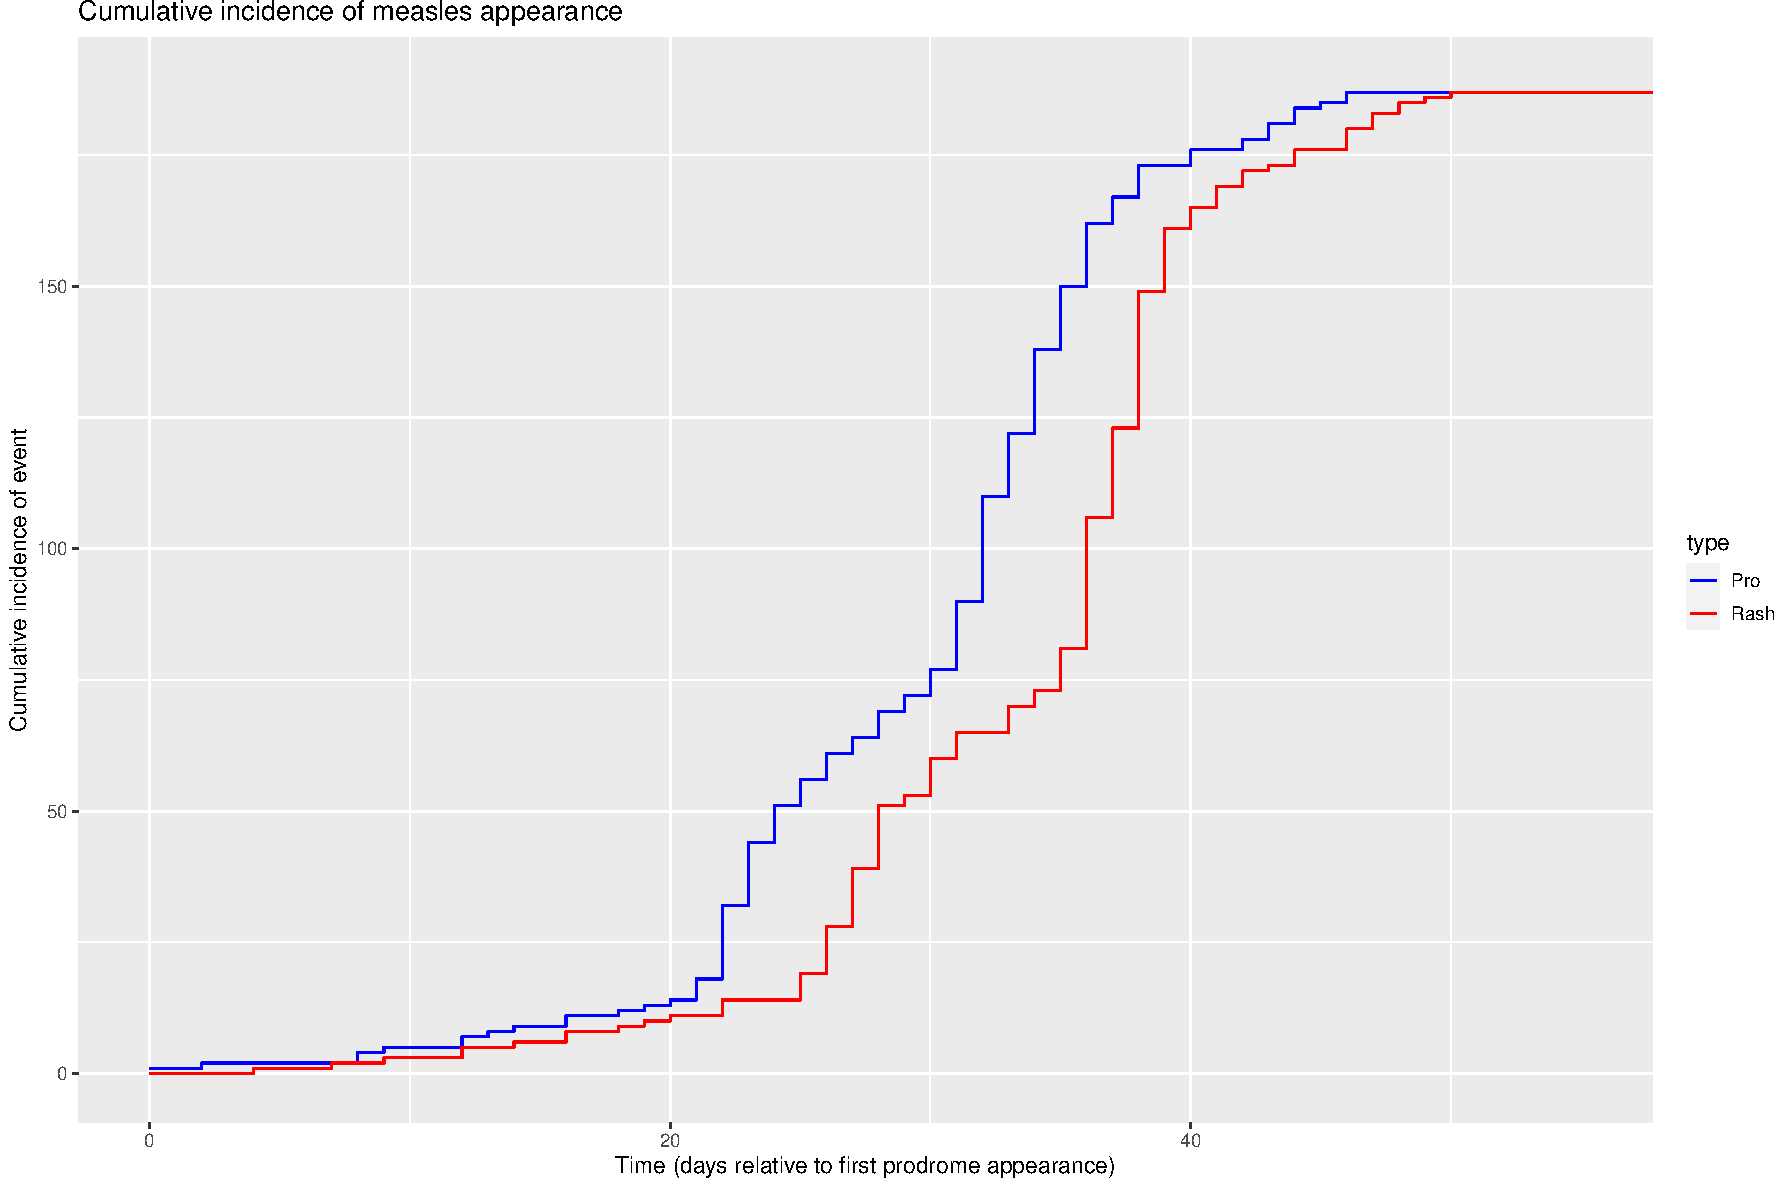
\includegraphics{Figs/unnamed-chunk-7-1} 

}

\caption{\label{fig:cifs}Empirical cumulative incidence functions of prodrome (symptom) onset and measles rash appearance.  We see that there is approximately a a constant lag between the two curves.}\label{fig:unnamed-chunk-7}
\end{figure}
\end{CodeChunk}

The real power of \code{agents_to_aggregate()} lies in its ability to
aggregate over any number of pre-specified states. For example, the
Hagelloch data sets contains two columns, \code{tI} and \code{tR}, the
time of infection and recovery, respectively of each individual. We can
then plot the SIR values through a time-invariant lens using
\pkg{ggplot2} and \pkg{ggtern} functions (as shown in Fig.
\ref{fig:hag-tern-raw}) or with our custom \code{geom},
\code{geom_aggregate}, which takes the raw agent data as input.

\begin{CodeChunk}
\begin{CodeInput}
R> hagelloch_sir <- hagelloch_raw %>%
+   agents_to_aggregate(states = c(tI, tR),
+                       min_max_time = c(0, 55)) %>%
+   rename(time = t, S = X0, I = X1, R = X2)
R> 
R> 
R> ggplot(hagelloch_sir, aes(x = S, y = I, z = R))+
+   coord_tern() +
+   geom_path() +
+   labs(x = "S", y = "I", z = "R",
+        title = "Time invariant view of Hagelloch measles outbreak") + 
+   theme_sir(base_size = 24)
\end{CodeInput}
\begin{figure}[H]

{\centering 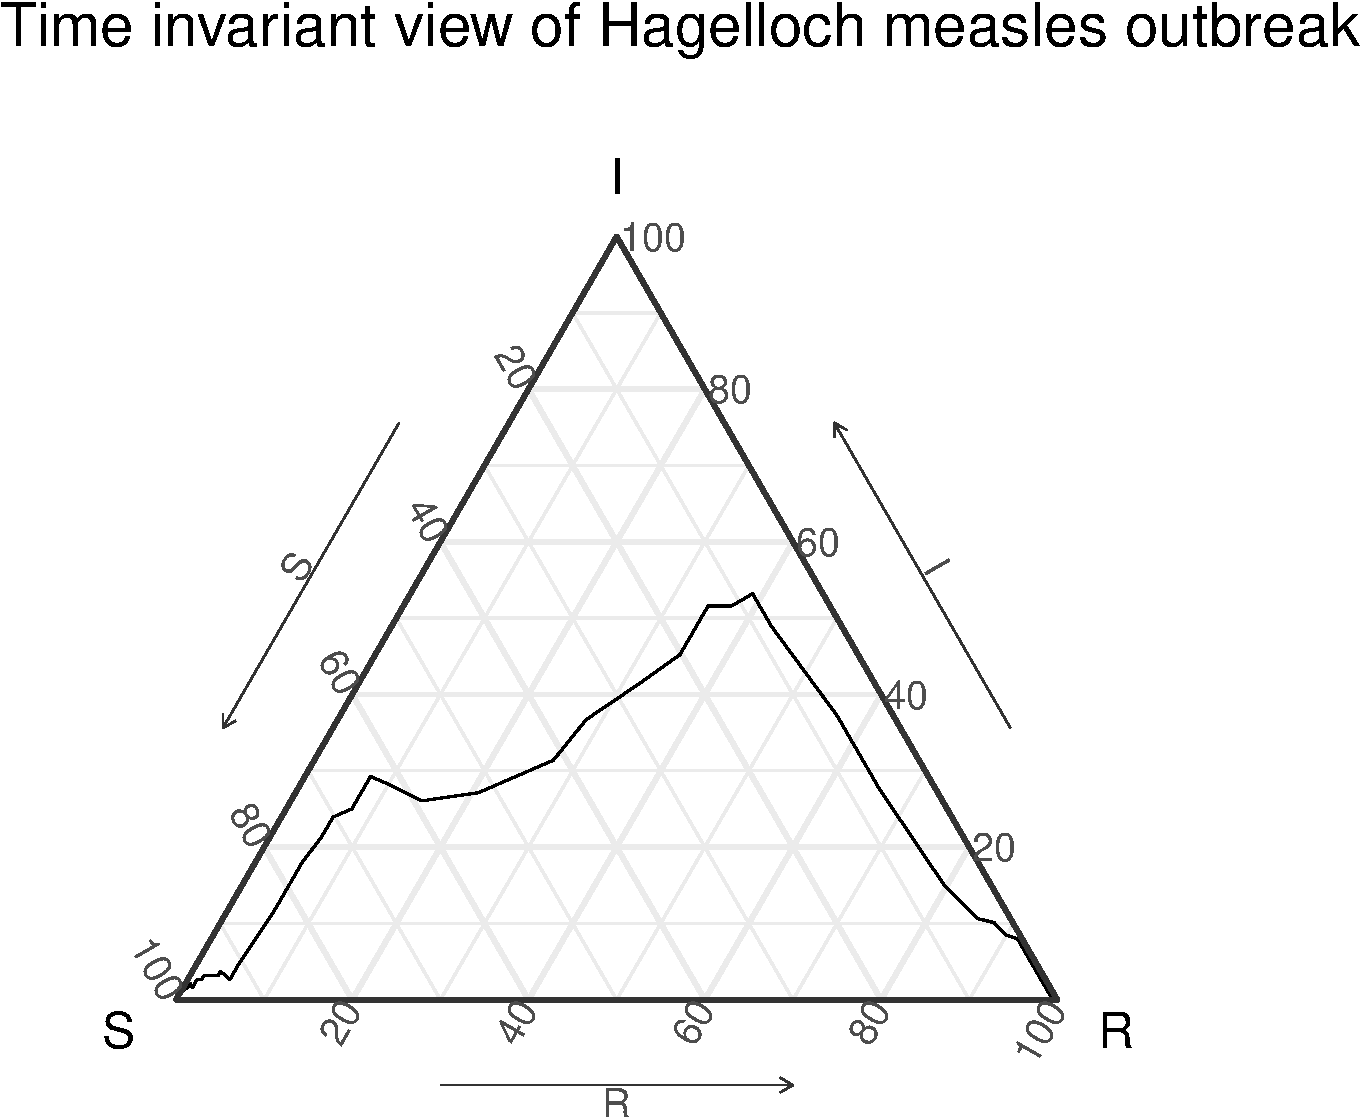
\includegraphics{Figs/unnamed-chunk-9-1} 

}

\caption{\label{fig:hag-tern-raw}Time invariant view of the Hagelloch epidemic where we view the individuals in Susceptible, Infectious, or Recovered states.  We see there are two peaks of infection (the vertical axis).}\label{fig:unnamed-chunk-9}
\end{figure}
\end{CodeChunk}

Moreover, we can look at the outbreaks of the disease by group within
\code{agent_to_aggregate()} or \code{geom_aggregate()}. This allows us
to examine differences among the different groups of individuals. For
example, we show the time invariant outbreak by class level in Figure
\ref{fig:tern-class-data}. Immediately, we see that time invariant
infection curve is different for the pre-school class compared to the
1st class. In the 1st class, we see about 95\% of the class become
infected and less than 10\% of them having recovered, which may be
indicative of a super-spreading event. This suspicion is further
confirmed in that 26 of the 30 1st class students have been reportedly
infected by the same individual.

\begin{CodeChunk}
\begin{CodeInput}
R> hagelloch_raw %>%
+   ggplot(aes(y = tI, z = tR, color = CL)) +
+   geom_aggregate(size = 2) + coord_tern() +
+   labs(x = "S", y = "I", z = "R",
+        color = "Class") +
+   scale_color_brewer(palette = "Dark2") +
+   facet_wrap(~CL)
\end{CodeInput}
\begin{figure}[H]

{\centering 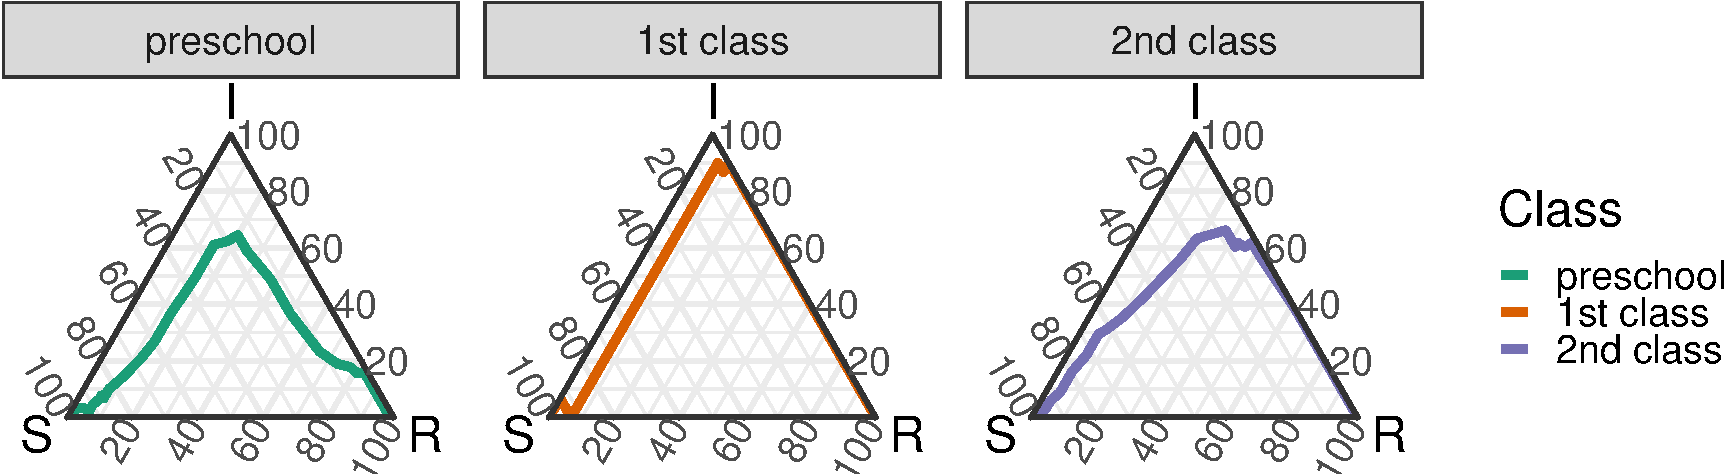
\includegraphics{Figs/unnamed-chunk-10-1} 

}

\caption{\label{fig:tern-class-data}Time invariant outbreak curves for the three class groups.  The pre-school class has a distinct peak of infection whereas the peak infection point for the other two classes are less well defined.}\label{fig:unnamed-chunk-10}
\end{figure}
\end{CodeChunk}

Along with multiple epidemic states, the function
\code{agents_to_aggregate} can also be extended to populations with
vital dynamics (e.g.~birth and death) and examples of this are shown in
the package vignette. In summary, \code{agents_to_aggregate()} is a
multi-purpose workhorse that may be leveraged to convert individual
level records into aggregate information that may be more useful for
some forms of epidemic modeling such as compartment modeling.

Up to this point, we have used \pkg{EpiCompare} in the context of
observed data. We also want to compare statistical models, and
\pkg{EpiCompare} aids in that process via a simple yet flexible
individual-level simulator, conversion tools for popular epidemic model
packages, and model assessments. We demonstrate an example here.

We first try to model the Hagelloch data with a stochastic SIR model,
which we refer to as the `simple SIR.' In our vignette, we show how to
fit this simple SIR model via maximum likelihood and simulate from the
model with those best fit parameters. Our function
\code{simulate_agents()} generates individual level data according to
discrete time multinomial draws, which depend on the number of
individuals in each state at the previous time step and a matrix of
transition probabilities. For example, the below code generates 100
simulations of an outbreak of a disease with one initial infector in a
population of \(n= 188\) individuals.

\begin{CodeChunk}
\begin{CodeInput}
R> trans_mat <- matrix(c("X0 * (1 - X1 * par1 / N)", "X0 * X1  * par1 / N", "0",
+                   "0", "X1 * (1 - par2)", "par2 * X1",
+                   "0", "0", "X2"), byrow = TRUE, nrow = 3)
\end{CodeInput}
\end{CodeChunk}

\begin{CodeChunk}
\begin{CodeInput}
R> set.seed(2020)
R> 
R> best_params <- c("beta" = .36, "gamma" = .13)
R> ## This is the SIR representation
R> 
R> rownames(trans_mat) <- c("S", "I", "R")
R> init_vals <- c(187, 1, 0)
R> par_vals <- c(par1 = best_params[1], par2 = best_params[2])
R> max_T <- 55
R> n_sims <- 100
R> 
R> agents <- simulate_agents(trans_mat,
+                        init_vals,
+                        par_vals,
+                        max_T,
+                        n_sims,
+                        verbose = FALSE)
\end{CodeInput}
\end{CodeChunk}

\begin{CodeChunk}
\begin{CodeInput}
R> agg_model <- agents %>% group_by(sim) %>%
+   agents_to_aggregate(states = c(I, R)) %>%
+   mutate(Type = "Simple SIR")
\end{CodeInput}
\end{CodeChunk}

The result of our simulation is the object \code{agents} which is a
18800 \(\times\) 5 data frame, which details the time of entry into the
\(S\), \(I\), and \(R\) states for a given simulation. Before we examine
the results of this simple SIR model, we will also examine another, more
sophisticated SIR model, this time from the package \pkg{EpiModel}.
Briefly, this model first fits a contact network to the set of
indivduals, where the class of the student is a covariate. The model
then simulates a SIR-epidemic on that network.

\begin{CodeChunk}
\begin{CodeInput}
R> library(EpiModel)
R> ## WARNING:  Will take a minute or two
R> 
R> set.seed(42)
R> nw <- network.initialize(n = 188, directed = FALSE)
R> nw <- set.vertex.attribute(nw, "group", rep(0:2, each = 90, 30, 68))
R> formation <- ~edges + nodematch("group") + concurrent
R> target.stats <- c(200, 300, 200)
R> coef.diss <- dissolution_coefs(dissolution = ~offset(edges),  duration = 5)
R> est1 <- netest(nw, formation, target.stats, coef.diss, edapprox = TRUE)
R> 
R> param <- param.net(inf.prob = 0.1, act.rate = 5, rec.rate = 0.1)
R> status.vector <- c(rep(0, 90), rep(0, 30), rep(0, 67), 1)
R> status.vector <- ifelse(status.vector == 1, "i", "s")
R> init <- init.net(status.vector = status.vector)
R> control <- control.net(type = "SIR", nsteps = 55,
+                        nsims = 100, epi.by = "group")
R> epimodel_sir <- netsim(est1, param, init, control)
\end{CodeInput}
\end{CodeChunk}

The output of this model is \code{epimodel_sir}, an object of class
\code{netsim}, which contains a plethora of modeling information. We
provide the function \code{fortify_aggregate()}, which can take objects
from specialized classes of modeling output and transform it into a
tidy-style data frame.

\begin{CodeChunk}
\begin{CodeInput}
R> fortified_net <- fortify_aggregate(epimodel_sir, 
+                                    states = c("s.num", "i.num", "r.num")) %>%
+   mutate(Type = "EpiModel SIR",
+          sim = as.numeric(gsub("sim", "", sim)))
\end{CodeInput}
\end{CodeChunk}

We can then analyze the results of the two models side by side as
time-invariant epidemic curves. The results are shown in Figure
\ref{fig:hag-simple-sir}, where a 90\% prediction band is estimated from
the delta ball method for each of the two models. For the Simple SIR
model, we see that the data generally covers the data fairly well but
clearly misses the second peak of infection. We also see that the
prediction band is very large, covering up a large area of the ternary
plot. On the other hand, for the \pkg{EpiModel} model, we see that the
prediction band covers the data quite well and takes up less area.

\begin{CodeChunk}
\begin{CodeInput}
R> both_models <- bind_rows(agg_model, fortified_net)
R> 
R> 
R> g <- ggplot() + geom_prediction_band(data = both_models %>% filter(t != 0),
+          aes(x = X0, y = X1, z = X2,
+               sim_group = sim, fill = Type),
+          alpha = .5,
+          conf_level = .90) 
\end{CodeInput}
\end{CodeChunk}

\begin{CodeChunk}
\begin{CodeInput}
R> g +   geom_path(data = both_models %>% filter(t !=0),
+             aes(x = X0, y = X1, z = X2, group = paste(Type, sim)),
+             alpha = .3, col = "gray40") + 
+     coord_tern() + theme_sir(base_size = 24) +
+   geom_point(data = hagelloch_sir,
+              aes(x = S, y = I, z =R), col = "black") +
+   labs(title = "Simple SIR model",
+        subtitle = "90% Prediction band and original data",
+        x = "S", y = "I", z = "R") +
+   scale_fill_manual(values = c("#006677", "#AA6600")) + 
+   facet_wrap(~Type) +
+   theme(legend.position = "bottom")
\end{CodeInput}
\begin{figure}[H]

{\centering 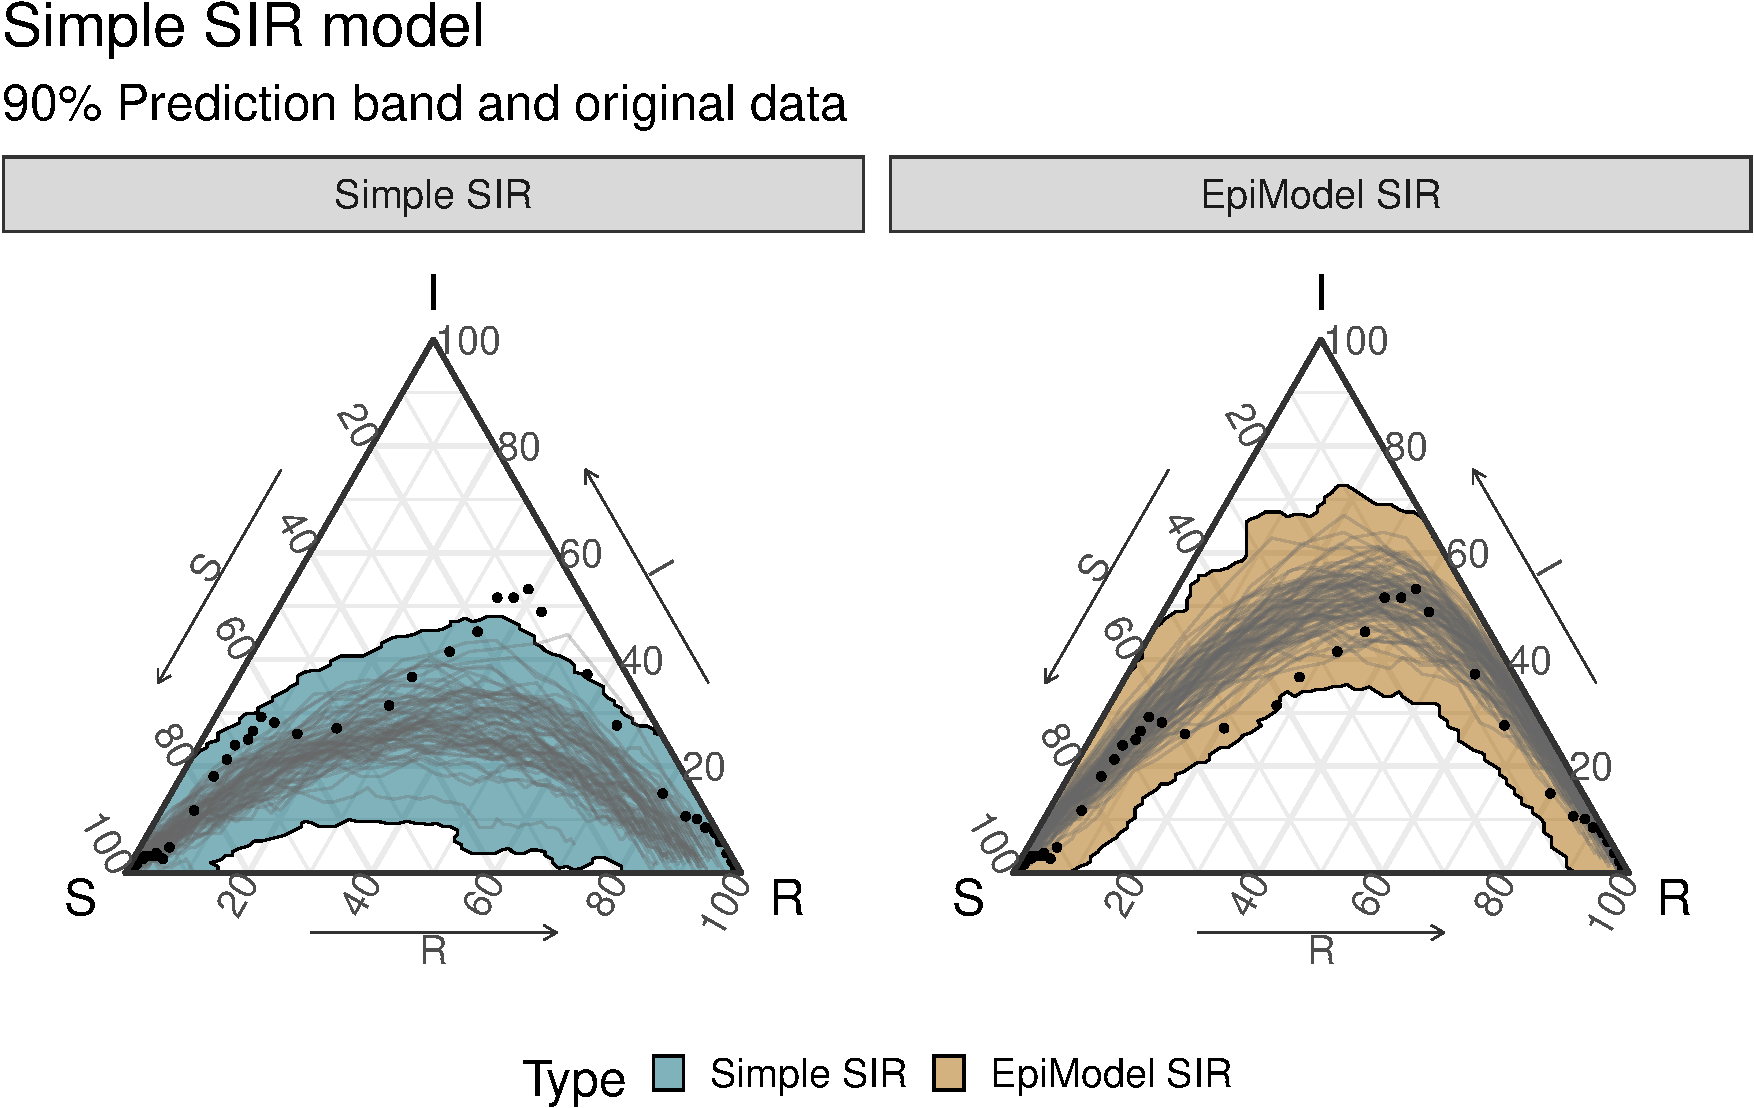
\includegraphics{Figs/unnamed-chunk-17-1} 

}

\caption{\label{fig:hag-simple-sir}  Original Hagelloch SIR data (black) along with 90\% prediction band and actual simulation paths from the Simple SIR and the EpiModel SIR models.}\label{fig:unnamed-chunk-17}
\end{figure}
\end{CodeChunk}

However, both models are not a good fit to the filamental path as
opposed to the individual points in \((S, I, R)\)-space. This can be
captured with the set of simulations both models predict (gray lines),
which all generally have a single defined peak of infection whereas the
data certainly looks like it has two distinct peaks, likely caused by
our assumed super-spreader event. This observation is backed up by the
below analysis that demonstrates that the estimated pseudo-density of
the observed epidemic (relative to the simulations from either model) is
much less likely then \textbf{any} of the simulations (reported in Table
\ref{tab:hags-extreme}). In conclusion, \pkg{EpiCompare} makes it clear
that, at a glance, 1) the \pkg{EpiModel} network model is a better fit
than the Simple SIR model, and 2) the fit is only good at the geometric
filamental level as opposed to the epidemic trajectory filamental level.

\begin{CodeChunk}
\begin{CodeInput}
R> #-- after cleaning up and combining --
R> all_together_df <- rbind(simple_sir,
+                          hagelloch_sir2)
\end{CodeInput}
\end{CodeChunk}

\begin{CodeChunk}
\begin{table}[!h]

\caption{\label{tab:cif-all-together-df}Top and bottom 2 rows of \tt{all\_together\_df}\text{, combining both simulated epidemics and the true epidemic.}}
\centering
\begin{tabular}[t]{lrrrrr}
\toprule
Type & sim & t & S & I & R\\
\midrule
Simple SIR & 1 & 0 & 188 & 0 & 0\\
Simple SIR & 1 & 1 & 187 & 1 & 0\\
true observation & 0 & 54 & 1 & 0 & 187\\
true observation & 0 & 55 & 1 & 0 & 187\\
\bottomrule
\end{tabular}
\end{table}

\end{CodeChunk}

\begin{CodeChunk}
\begin{CodeInput}
R> compression_df <- all_together_df %>% group_by(Type, sim) %>% 
+   filament_compression(data_columns = c("S","I","R"), 
+                        number_points = 20)
\end{CodeInput}
\end{CodeChunk}

\begin{CodeChunk}
\begin{CodeInput}
R> tdmat <- compression_df %>% 
+   dist_matrix_innersq_direction(
+     position = c(1:length(compression_df))[
+       names(compression_df) %in% c("S","I", "R")],
+     tdm_out = T)
R> 
R> simple_sir_true_obs_info <- tdmat %>% 
+   compare_new_to_rest_via_distance(
+     new_name_id = data.frame(Type = "true observation", sim = 0),
+     distance_func = distance_psuedo_density_function, 
+     sigma = "20%") 
\end{CodeInput}
\end{CodeChunk}

\begin{CodeChunk}
\begin{table}[!h]

\caption{\label{tab:hags-extreme}The extremeness of the true simulations based on comparing psuedo-density estimates between true vs simulated curves}
\centering
\begin{tabular}[t]{l>{\raggedleft\arraybackslash}p{6cm}>{\raggedleft\arraybackslash}p{6cm}}
\toprule
Type & simulations-based estimated psuedo-density & proportion of simulations with lower estimated psuedo-density\\
\midrule
Simple SIR & 0.0117621 & 0.01\\
EpiModel SIR & 0.0356503 & 0.01\\
\bottomrule
\end{tabular}
\end{table}

\end{CodeChunk}

Overall, \pkg{EpiCompare} aids in the data analysis pipeline for both
novice and expert practitioners and coders alike. These tools encourage
model and simulation exploration of many of the existing and
well-supported packages that already exist, and side-by-side comparison
thereof. Finally, we hope that practicioners will consider using
time-invariant analysis when trying to assess and compare epidemics and
epidemic models.

\hypertarget{a.-appendix}{%
\section*{A. Appendix}\label{a.-appendix}}
\addcontentsline{toc}{section}{A. Appendix}

\hypertarget{a.1-proof-of-theorem}{%
\subsection*{\texorpdfstring{A.1 Proof of Theorem
\ref{thm:sir-scale}}{A.1 Proof of Theorem }}\label{a.1-proof-of-theorem}}
\addcontentsline{toc}{subsection}{A.1 Proof of Theorem
\ref{thm:sir-scale}}

\begin{proof}\label{proof:thm}
\cite{Harko2014} provide an analytical solution for the Kermack and McKendrick equations (Eq. \eqref{eq:sir-ode}) by reparameterizing the ODEs so that $\mathcal{S}(u) = S(t)$, $\mathcal{I}(u) = S(t)$, and $\mathcal{R}(u) = R(t)$ for $0< u_T < 1$ with
\begin{align}\label{eq:harko-odes}
\mathcal{S}(u) &= S(0)u\\
\mathcal{I}(u) &= N - R(0) + NR_0^{-1}\log u - S(0)u \nonumber\\
\mathcal{R}(u) &= R(0) - NR_0^{-1} \log u, \nonumber
\end{align}
and $u$ and t are related by the following integral,
\begin{align*}
    t &= \int_{u}^1 \frac{N}{\beta \tau (N - R(0) + R_{0}^{-1} \log \tau - S(0)\tau)}d\tau \\
    &= \int_{u}^1 \frac{1}{\beta f(S(0), R(0), N, R_0, \tau)} d \tau\\
    &= \int_{u}^1 \frac{1}{\beta f(\tau)} d\tau,
\end{align*}
where we have made the denominator of the integral a function of $N$, the initial values, $R_0$, and $\tau$, which we further condense to $f(\tau)$ for brevity.
Then for a given $t$ we want to find $s$ such that $(S_1(t), I_1(t), R_1(t)) = (S_2(s), I_2(s), R_2(s))$.  Or equivalently, for a fixed $u$ want to find $v$ such that  $\mathcal{S}_1(u) = \mathcal{S}_2(v)$ and then the corresponding $t$ and $s$ are given by
\begin{align*}
    t & = \int_{u}^1 \frac{1}{\beta_1 f(\tau)} d\tau \\
    s & = \int_{v}^1 \frac{1}{\beta_2 f(\tau)} d\tau.
\end{align*}
Note that since the equations in Eq. \eqref{eq:harko-odes} are functions of the initial values and $R_0$, then $u = v$. We then can find a relation for $s$,
    \begin{align*}
    s & = \int_{u}^1 \frac{1}{\beta_2 f(\tau)} d\tau  \\
    & = \int_{u}^1 \frac{1}{a\beta_1 f(\tau)} d\tau \\ 
    &= \frac{1}{a}\int_{u}^1 \frac{1}{\beta_1 f(\tau)} d\tau \\
    &= \frac{1}{a}t.
\end{align*}
\end{proof}

\bibliography{EpiCompare.bib}


\end{document}

